% Project 3B: hemodynamic attenuation. Standalone-compilable; to drop into the thesis, keep the
% body and merge the \bibitem entries into the thesis bibliography.
%
% Numbers come from the runs in results/ (figures drawn by experiments/figure_main.py,
% figure_setup.py and figure_induction.py). Astrocyte equations are quoted from Kozachkov,
% Kastanenka & Krotov (PNAS 2023), Eqs. 6-11.

\documentclass[11pt]{report}
\usepackage[margin=1.1in]{geometry}
\usepackage{amsmath,amssymb,booktabs,graphicx,microtype}
\usepackage[T1]{fontenc}
\usepackage[font=small,labelfont=bf]{caption}
\usepackage{xcolor}
\usepackage{hyperref}
\hypersetup{colorlinks=true,allcolors=blue!55!black}
\graphicspath{{../figures/}}

\newcommand{\kstar}{k^\star}
\newcommand{\Ltriv}{L_{\mathrm{triv}}}

\begin{document}
\setcounter{chapter}{5}
\chapter{Hemodynamic Attenuation of Attention Heads}
\label{ch:hemo}

%=========================================================================================
\section{Introduction}

Earlier chapters used blood flow as data, training models to read hemodynamic signals. This
chapter uses blood flow as a design principle: the way the brain decides which vessels to keep
is used to decide which attention heads a transformer keeps.

In Chapter~4, a trained transformer carried its causal computation in two of forty heads, but
this was found only after training, by ablating each head in turn, and the number of heads to
keep had to be chosen by hand. This chapter asks whether a model can find the number of heads it
needs during training, without being given it. We introduce a rule for this, hemodynamic
attenuation, and test it on a task whose minimal number of heads is known.

%=========================================================================================
\section{Background}

\subsection{Blood supply}

Four properties of cerebral blood supply motivate the rule:
\begin{enumerate}
\item Supply follows need: local blood flow rises with neural activity, signalled in part by
      astrocytes \cite{attwell2010}. Each head is given a valve $g_h \in [0,1]$.
\item A vessel is dispensable when collateral vessels can supply its tissue \cite{faber2014}.
      A head is valued by what is lost when it closes and the other heads compensate, its
      collateral value.
\item Maintaining a vessel has a metabolic cost \cite{murray1926}. Each open head has a fixed
      price; there is no target number of heads.
\item Unneeded vessels regress gradually \cite{chen2012,franco2015}, and collaterals can enlarge
      when a route is blocked \cite{faber2014}. Closing heads fade out over 100 steps and can
      be reopened.
\end{enumerate}
The biology motivates the design; no claim is made about the brain.

\subsection{Astrocytes and attention}

Kozachkov et al.\ \cite{kozachkov2023} showed that neurons and one astrocyte can approximately
compute self-attention. With hidden activity $h = \varphi(Wx) \in \mathbb{R}^m$ and output
synapses $H \in \mathbb{R}^{d \times m}$, each scaled by an astrocyte process (their Eq.~6),
\begin{equation}
\ell = \big(H \odot \widetilde P\big)\, h + x,
\qquad \widetilde P_{i\alpha} = 1/p_{i\alpha}.
\label{eq:koz6}
\end{equation}
Calcium equalises across the astrocyte, so every process takes the same value (their Eq.~8) and
$H \odot \widetilde P = H/p$ with $p = \frac{1}{m}\sum_j \varphi(k_j)^{\top}\varphi(q_t)$. With
Hebbian weights $H = \frac{1}{m} V\varphi(K)^{\top}$, the output for token $t$ is (their Eq.~11)
\begin{equation}
\ell_t = \frac{V\,\varphi(K)^{\top}\varphi(q_t)}{\sum_j \varphi(k_j)^{\top}\varphi(q_t)} + x_t
\;\approx\; \sum_i \frac{e^{k_i^{\top} q_t}}{\sum_j e^{k_j^{\top} q_t}}\, v_i + x_t ,
\end{equation}
since $\varphi(a)^{\top}\varphi(b) \approx e^{a^{\top} b}$. The neurons compute the numerator of
the softmax and the astrocyte its denominator.

\subsection{Head pruning}

Michel et al.\ \cite{michel2019sixteen} remove heads by a gradient score, and Voita et al.\
\cite{voita2019analyzing} learn head gates with an $L_0$ penalty. Optimal Brain Damage \cite{obd}
scores a parameter by the loss increase when it is removed; Optimal Brain Surgeon \cite{obs} by
the increase after the remaining parameters are re-fitted. ZipLM \cite{ziplm} applies the latter to
whole heads of trained language models. All of these prune after training, to a size chosen by
the user.

%=========================================================================================
\section{Methods}

\subsection{Task}

\begin{figure}[t]
\centering
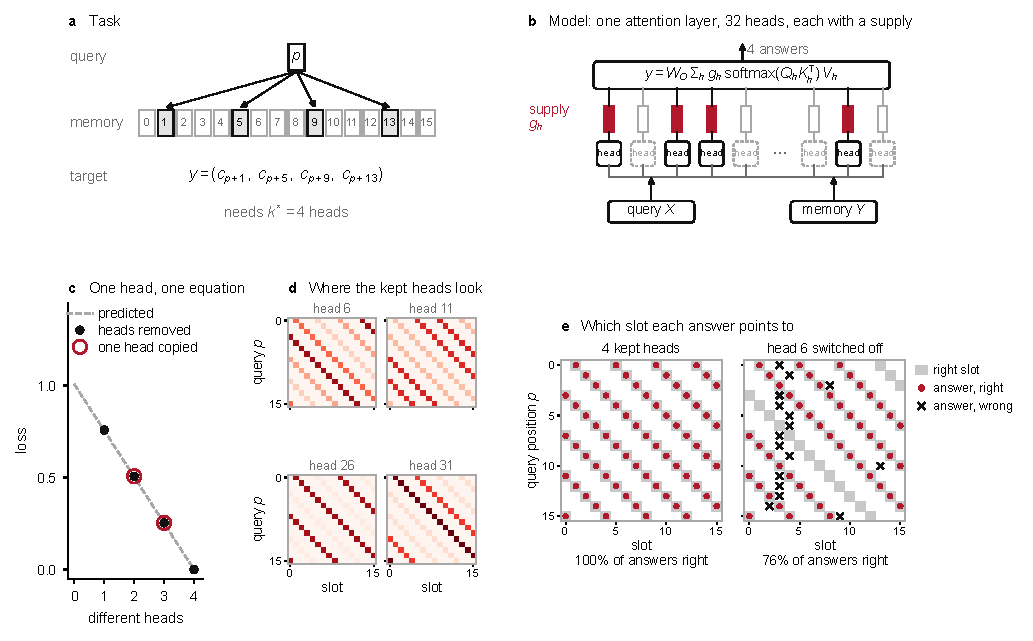
\includegraphics[width=\linewidth]{fig_setup.pdf}
\caption{Task and model.
\textbf{a}, A query carries a position $p$; the target is the items stored $1, 5, 9, 13$ slots
ahead, so 4 heads are needed.
\textbf{b}, One attention layer with 32 heads, each with a valve $g_h$; filled valves are open.
\textbf{c}, Loss with $k$ different heads on a trained 4-head model, against the prediction
$1 - k/4$.
\textbf{d}, The slot each answer points to: all correct with the 4 kept heads, 76\% with head 6
switched off.}
\label{fig:setup}
\end{figure}

The memory has $N = 16$ slots, each holding a random item $c_j$. A query specifies a position
$p$, and the target is the items at $R$ fixed offsets (Figure~\ref{fig:setup}a):
\begin{equation}
\text{target}(p) = \big(c_{p+\delta_1},\ \dots,\ c_{p+\delta_R}\big),
\qquad \text{slots modulo } N.
\end{equation}
Items are redrawn for every example, so the model must learn where to attend.

A head returns, for each query, one weighted average of the items: one linear equation in the
$R$ unknown items. Recovering $R$ items needs $R$ independent equations, so the task needs
$\kstar = R$ heads, and with $k < R$ heads the lowest achievable loss is
\begin{equation}
\text{loss}(k) = \Big(1 - \frac{k}{R}\Big)\, \Ltriv,
\label{eq:law}
\end{equation}
where $\Ltriv$ is the loss of predicting the mean. Duplicate heads give the same equation and
count once. Measured losses agree with Equation~\eqref{eq:law} to within 1\%
(Figure~\ref{fig:setup}c).

The task counts as solved when the loss is below $0.02\,\Ltriv$. Trained models sit hundreds of
times below this threshold, and losing one needed head raises the loss by about $\Ltriv/R$, so
results are unchanged for any threshold from $0.01$ to $0.1$.

\subsection{Model}

Matrices have one column per token, following \cite{kozachkov2023}. The model is one
cross-attention layer with $H = 32$ heads and no MLP, reading queries $X$ and memory $Y$. Head $h$
computes
\begin{equation}
E_h = \exp\!\Big(\tfrac{1}{\sqrt{d_k}}\, (W_K^h Y)^{\top} W_Q^h X\Big),
\qquad
D_h = \operatorname{diag}\big(\mathbf{1}^{\top} E_h\big),
\qquad
O_h = W_V^h Y\, E_h\, D_h^{-1},
\end{equation}
where $E_h D_h^{-1}$ is the softmax. Each head is scaled by its valve before the heads are
combined:
\begin{equation}
\hat{T} = \sum_{h=1}^{H} g_h\, W_O^h\, O_h = \big(W_O \odot P\big)\, O,
\qquad P_{i,(h,c)} = g_h .
\label{eq:valve}
\end{equation}
A head with $g_h = 0$ contributes nothing and receives no gradient, so a model with $k$ open
valves is exactly a $k$-head model.

The right-hand form of Equation~\eqref{eq:valve} is the astrocyte gain of
Equation~\eqref{eq:koz6}, constant within each head's block of $W_O$ rather than over a whole
domain. The layer therefore contains two gains of the same form (Table~\ref{tab:astro}):
\begin{equation}
\hat T = \sum_h g_h\, W_O^h\, W_V^h Y\, E_h\, D_h^{-1},
\end{equation}
where $D_h^{-1}$ is the per-query gain the astrocyte computes in \cite{kozachkov2023} and $g_h$ is
the per-head gain set by our rule. The correspondence is algebraic only.

\begin{table}[h]
\centering
\small
\begin{tabular}{lll}
\toprule
 & Astrocyte gain \cite{kozachkov2023} & Head valve \\
\midrule
Matrix form & $H \odot \widetilde P$, one value $1/p$ & $W_O \odot P$, one value $g_h$ per head \\
Set by      & pooled input activity                   & collateral value relative to a price \\
Time scale  & every token                             & over training \\
Function    & softmax normalisation                   & selection of heads \\
\bottomrule
\end{tabular}
\caption{Two gains on blocks of synapses.}
\label{tab:astro}
\end{table}

\subsection{Hemodynamic attenuation}
\label{sec:rule}

All valves start open. After a warm-up of 10\% of training, every 25 steps the rule (1) computes
the collateral value of every open head, (2) closes the lowest-valued head if its value is below
the price $0.03\,\Ltriv$, and (3) reopens the highest-valued closed head if its value exceeds twice
the price. A closing valve decreases by $1/100$ per step.

The collateral value is the increase in the best-fit loss when head $h$ is removed and the other
open heads re-fit their output weights:
\begin{equation}
v_h = \min_W L(\text{without } h) - \min_W L(\text{all open heads}).
\end{equation}
With $Z$ the stacked outputs of the open heads on a batch, $A = \frac{1}{n} ZZ^{\top}$,
$W^{*} = \frac{1}{n} TZ^{\top}A^{-1}$, $M = A^{-1}$ and $J$ the rows of head $h$,
\begin{equation}
v_h = \tfrac{1}{d_{\text{out}}}\,
\operatorname{tr}\!\big( W^{*}_J \,(M_{JJ})^{-1} W^{*\top}_J \big),
\end{equation}
one inverse for all heads. This is the block Optimal Brain Surgeon score \cite{obs,ziplm}; the
contribution is its use during training, with a price, a gradual fade, and reopening.

The re-fit is what makes a copy worthless. If $z_2 = z_1$ and the target is $z_1$, removing head 2
without re-fitting raises the loss by $0.25\,\mathrm{var}(z_1)$ when the weights are
$(0.5, 0.5)$; with re-fitting head 1 takes weight 1 and $v_2 = 0$. Computing the values added
about 5\% to training compute. In one layer $A$ is the exact curvature; deeper models would need a
layer-wise approximation \cite{ziplm}.

\subsection{Baselines and evaluation}

All methods share the model, task, training and runs. Published methods, run inside our
training: ZipLM-style \cite{ziplm} (the same score applied once, then fine-tuning), Michel et al.\
\cite{michel2019sixteen}, and Voita et al.\ \cite{voita2019analyzing}. Controls remove one part of
the rule: no fade, no re-fit (the Optimal Brain Damage score \cite{obd}), and no score (random
choice).

We report exact count (open heads over the last 40\% of training equal $\kstar$) and never broke
(after first falling below the solved threshold, the loss never exceeds it). Experiments use
$\kstar = 2, 4, 8$ with 10 seeds each, plus runs with duplicated heads, runs with random head
failure, and a two-layer induction task \cite{olsson2022}.

%=========================================================================================
\section{Results}

\begin{figure}[t]
\centering
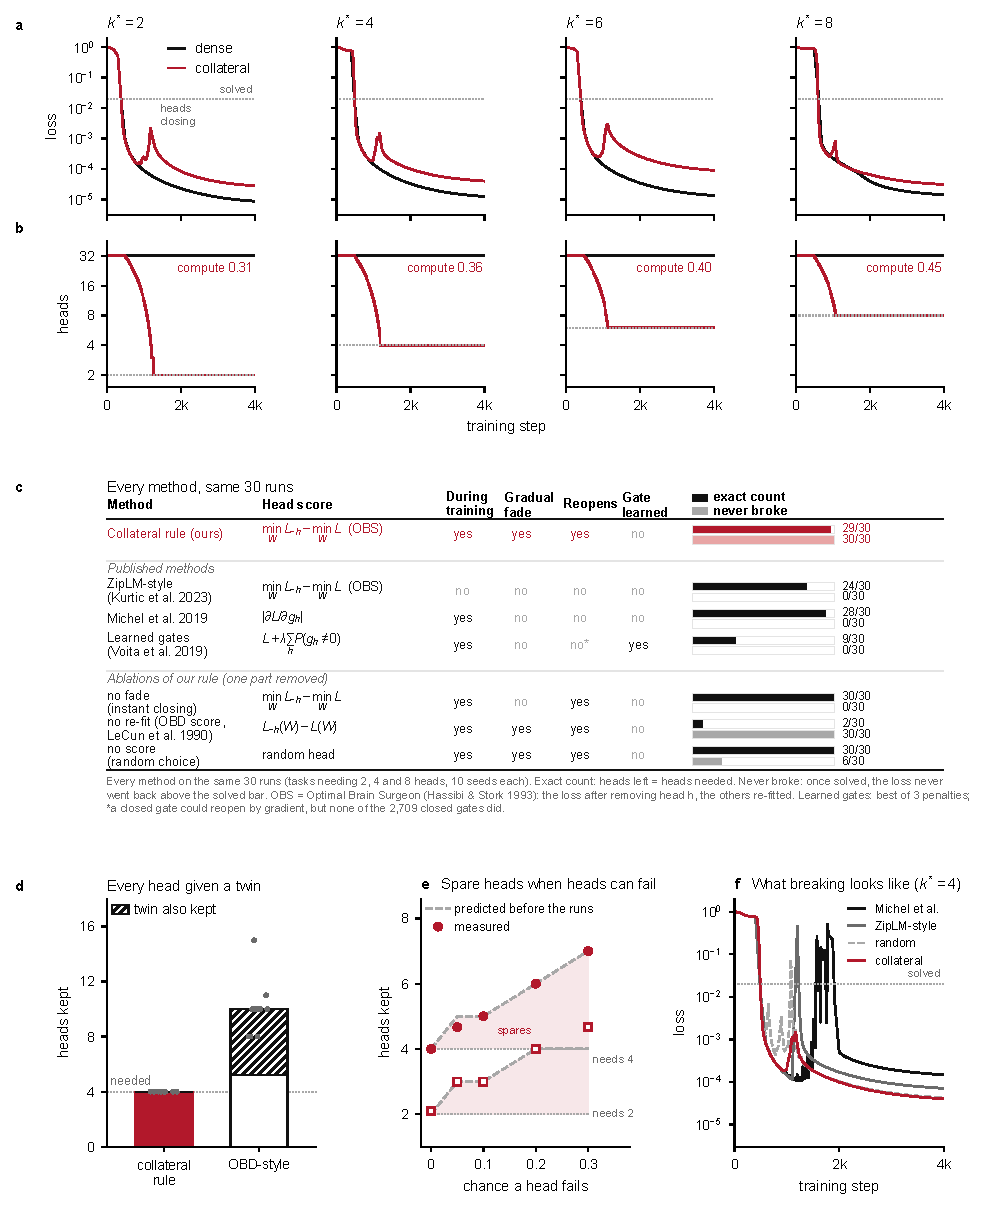
\includegraphics[width=\linewidth]{fig_main.pdf}
\caption{Hemodynamic attenuation during training.
\textbf{a}, Loss of the dense model (black) and with hemodynamic attenuation (red).
\textbf{b}, Open heads; dotted line, $\kstar$.
\textbf{c}, All methods on the same 30 runs.
\textbf{d}, Runs in which every head starts with an identical copy.
\textbf{e}, Spare heads kept under random failure, against the prediction.
\textbf{f}, One run per method; only hemodynamic attenuation stays below the solved threshold.}
\label{fig:main}
\end{figure}

\begin{table}[h]
\centering
\small
\begin{tabular}{lcc}
\toprule
Method (30 runs each) & Exact count & Never broke \\
\midrule
Hemodynamic attenuation & 29/30 & 30/30 \\
\addlinespace
ZipLM-style \cite{ziplm}               & 24/30 & 0/30 \\
Michel et al.\ \cite{michel2019sixteen} & 28/30 & 0/30 \\
Voita et al.\ \cite{voita2019analyzing} & 9/30  & 0/30 \\
\addlinespace
No fade                                & 30/30 & 0/30 \\
No re-fit                              & 2/30  & 30/30 \\
No score (random)                      & 30/30 & 6/30 \\
\bottomrule
\end{tabular}
\caption{Exact count and stability on the retrieval task ($\kstar = 2, 4, 8$, 10 seeds each).}
\label{tab:results}
\end{table}

\paragraph{Count and stability.} Hemodynamic attenuation kept exactly $\kstar$ heads in 29 of 30
runs and never broke the model in 30 of 30; no other method achieved both
(Table~\ref{tab:results}). Without the fade the model broke in every run; without the re-fit it
kept too many heads; with random choice it broke in 24 of 30 runs.

\paragraph{Duplicated heads.} With every head starting as a copy of another, the rule kept 4 heads
and never both members of a pair; without the re-fit, 8 to 15 heads and 4 to 7 pairs were kept
(Figure~\ref{fig:main}d).

\paragraph{Backup heads.} If each head fails with probability $p$, a head's value with $B$ heads
open is
\begin{equation}
v(B) = \frac{1-p}{R}\; \Pr\big[\,\text{Binomial}(B-1,\,1-p) \le R-1\,\big],
\end{equation}
and the rule should keep the largest $B$ with $v(B)$ above the price. This prediction, made before
the experiments, matched 21 of 24 runs exactly and the rest to within one head
(Figure~\ref{fig:main}e).

\paragraph{Induction.} In a two-layer attention-only model with 8 + 8 heads, trained to predict
the token that followed an earlier copy of the current token, the minimal circuit is one
previous-token head and one induction head \cite{olsson2022}. Hemodynamic attenuation kept
2 + 1 heads in 10 of 10 runs, one more than the minimum, and never broke the model; the kept heads
had the expected roles in all 10 runs, and switching off the induction head reduced next-token
accuracy on the repeat to zero (Figure~\ref{fig:induction}). On this task every method kept the
same 2 + 1 heads, so only stability separated them: the method of Michel et al.\ broke the model
in all 10 runs, while the controls without re-fit or with random choice did not.

\begin{figure}[t]
\centering
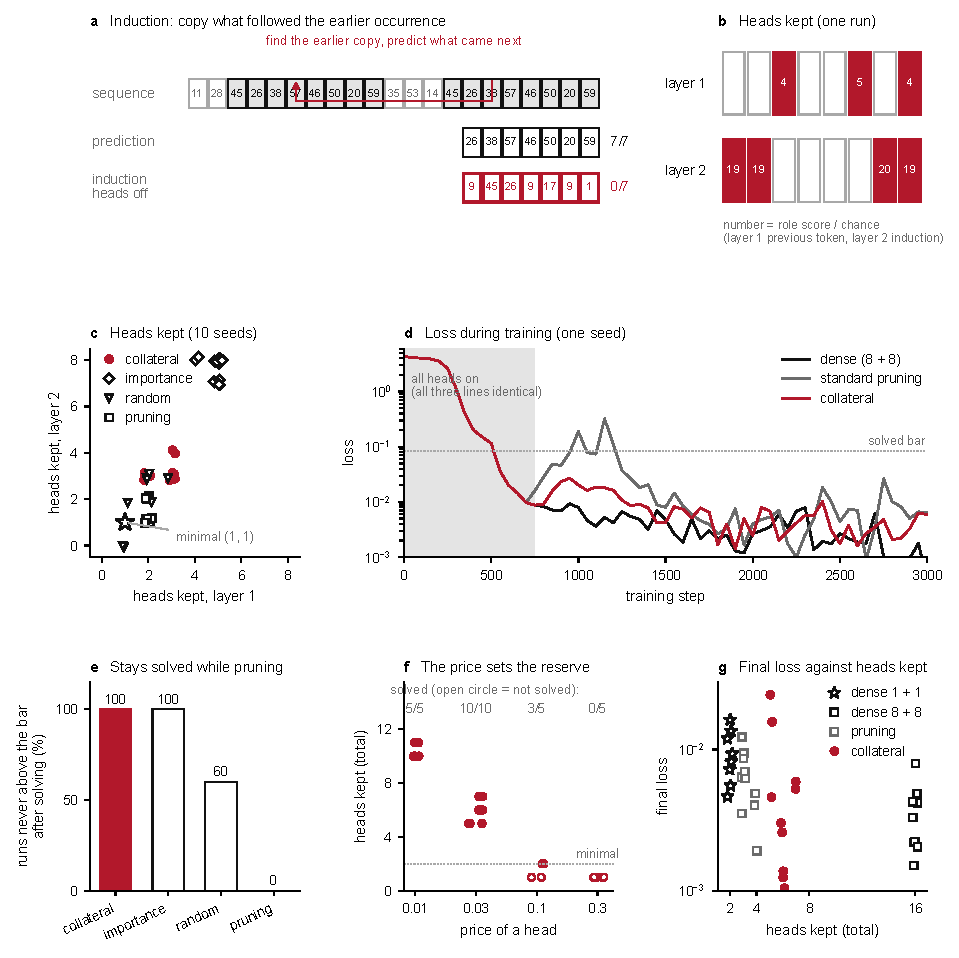
\includegraphics[width=\linewidth]{fig_induction.pdf}
\caption{Two-layer induction.
\textbf{a}, An example sequence and the model's predictions on the repeat, with all kept heads
(7/7 correct) and with the layer-2 head switched off (0/7).
\textbf{b}, Heads kept in one run; numbers give how much more than chance each head attends to the
position its role requires.
\textbf{c}, Runs that never broke, 10 per method, all with the same settings. Every run kept 2 + 1
heads.
\textbf{d}, Loss during training for one seed.}
\label{fig:induction}
\end{figure}

\paragraph{Cost.} Final loss was 2 to 7 times the dense model's, well below the threshold, using
0.31 to 0.45 of its head-steps. The saving is nominal, since closed heads are still computed.

%=========================================================================================
\section{Discussion}

A rule built from how vessels are maintained and pruned recovered a known minimal circuit during
a single training run, without being given its size and without the model leaving the solved
regime. Removing any one of its components lost either the count or stability.

The tasks are small and the main model has one layer, which is what makes the answer known; the
results do not yet extend to large language models. The collateral value is exact only for one
layer, and the compute saving requires skipping closed heads in code. The biology motivates the
rule but is not evidence for it.

Two experiments would connect this chapter to the rest of the thesis and have not yet been run:
applying the rule to qSA-Cross, to test whether it keeps the two causal heads found in Chapter~4,
and to the Cross-Site Transformer on WildPPG, to test whether the same heads are kept across all
sixteen leave-one-subject-out folds.

%=========================================================================================
\begin{thebibliography}{99}
% Check volume and page details against the originals before submission.
\bibitem{kozachkov2023} L.~Kozachkov, K.~V.~Kastanenka, D.~Krotov. Building transformers from
  neurons and astrocytes. \emph{PNAS} 120(34):e2219150120, 2023.
\bibitem{attwell2010} D.~Attwell, A.~M.~Buchan, S.~Charpak, M.~Lauritzen, B.~A.~MacVicar,
  E.~A.~Newman. Glial and neuronal control of brain blood flow. \emph{Nature} 468:232--243, 2010.
\bibitem{faber2014} J.~E.~Faber, W.~M.~Chilian, E.~Deindl, N.~van Royen, M.~Simons. A brief
  etymology of the collateral circulation. \emph{Arterioscler.\ Thromb.\ Vasc.\ Biol.}
  34(9):1854--1859, 2014.
\bibitem{murray1926} C.~D.~Murray. The physiological principle of minimum work: I.\ The vascular
  system and the cost of blood volume. \emph{PNAS} 12(3):207--214, 1926.
\bibitem{chen2012} Q.~Chen et al. Haemodynamics-driven developmental pruning of brain
  vasculature in zebrafish. \emph{PLoS Biol.} 10(8):e1001374, 2012.
\bibitem{franco2015} C.~A.~Franco et al. Dynamic endothelial cell rearrangements drive
  developmental vessel regression. \emph{PLoS Biol.} 13(4):e1002125, 2015.
\bibitem{obd} Y.~LeCun, J.~S.~Denker, S.~A.~Solla. Optimal brain damage. \emph{NeurIPS} 2, 1989.
\bibitem{obs} B.~Hassibi, D.~G.~Stork, G.~J.~Wolff. Optimal brain surgeon and general network
  pruning. \emph{IEEE International Conference on Neural Networks}, 1993.
\bibitem{ziplm} E.~Kurtic, E.~Frantar, D.~Alistarh. ZipLM: Inference-aware structured pruning
  of language models. \emph{NeurIPS}, 2023.
\bibitem{michel2019sixteen} P.~Michel, O.~Levy, G.~Neubig. Are sixteen heads really better than
  one? \emph{NeurIPS}, 2019.
\bibitem{voita2019analyzing} E.~Voita, D.~Talbot, F.~Moiseev, R.~Sennrich, I.~Titov. Analyzing
  multi-head self-attention: specialized heads do the heavy lifting, the rest can be pruned.
  \emph{ACL}, 2019.
\bibitem{olsson2022} C.~Olsson et al. In-context learning and induction heads.
  \emph{Transformer Circuits Thread}, 2022.
\end{thebibliography}

\end{document}
